\section{Time box 5} 
\listoftodos
\subsection{Time box planning}
\begin{figure}[H]
	\begin{centering}
		\missingfigure{Updated timebox figure}
		%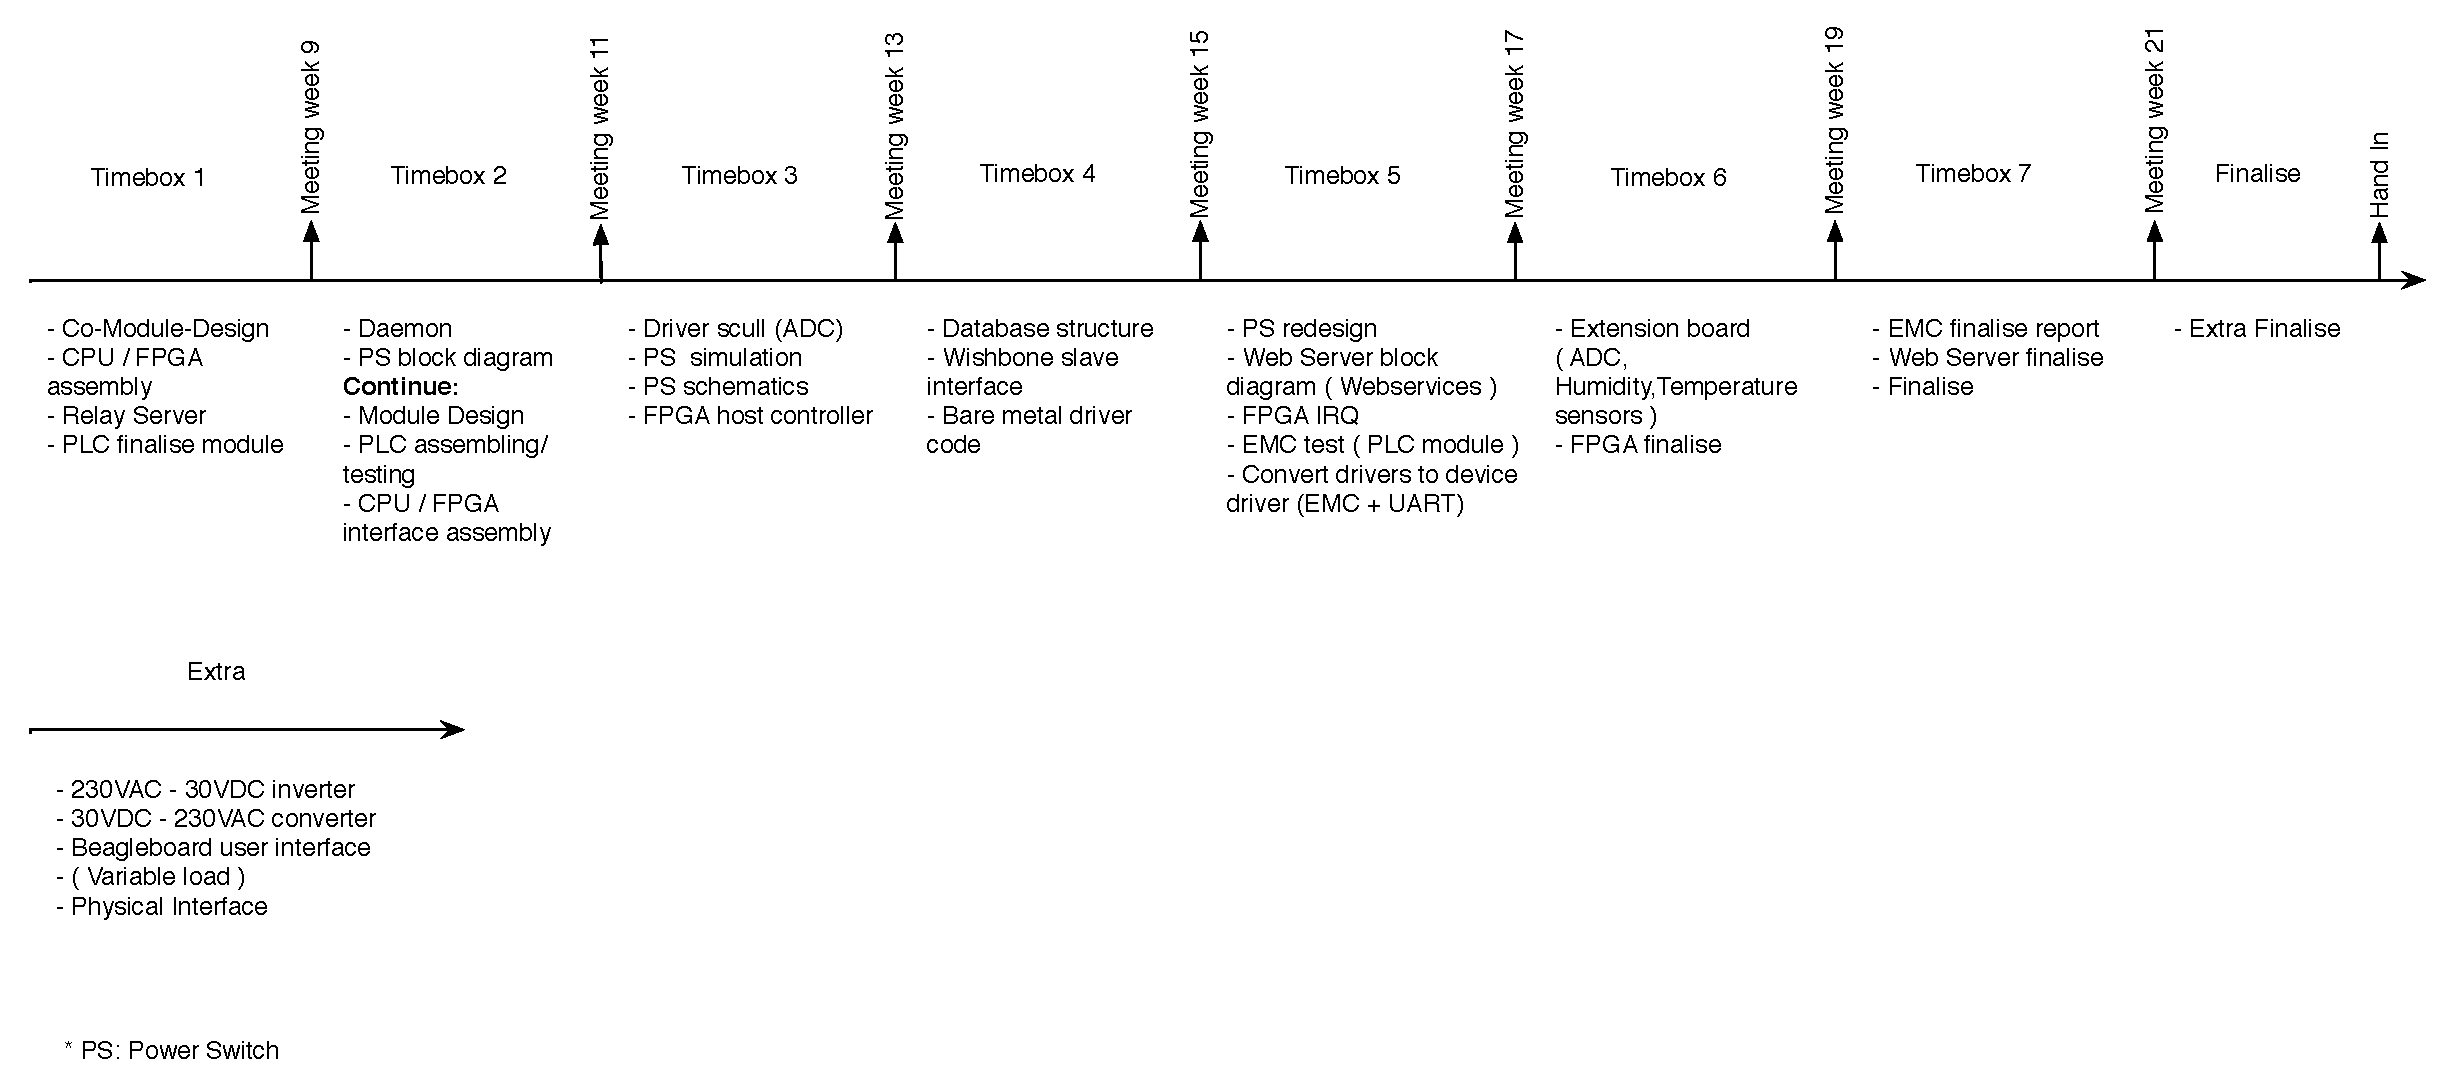
\includegraphics[width=1.0\textwidth]{images/tb_r4.pdf}
		%\caption{Updated time-box}
	\end{centering}
\end{figure}
\subsubsection{Work to be done in this time box}
\begin{itemize}
	\item Power Switch module redesign
	\begin{itemize}
		\item Improvements
		\item Simulation
		\item Redesign
	\end{itemize}
	\item UART Device driver
		\begin{itemize}
			\item Convert UART bare-metal driver into Linux device driver
		\end{itemize}
	\item Interrupt register
	\begin{itemize}
		\item Wishbone slave interface
		\item Interrupt signals
		\item Interrupt handling
	\end{itemize}
\end{itemize}
\paragraph{Description:}
\begin{description}
	\item[UART Device driver] Convert the bare-metal UART driver from the last time box into a device driver, in order to be able to access the UART hardware from user space in the uClinux environment.
	\item[Power Switch] Main component of the energy hub system, controls the ports for each module allowing energy to flow in both directions.
	\item[Interrupt register] is a block in the Spartan 6, that is allow to interrupt the ARM7 directly. The register is handling other interrupts from the Spartan 6 and tell the ARM7 where the interrupt came from.
\end{description}
\subsubsection{Time planning}
\begin{table}[H]
\centering
%	\todo[inline]{Update time}
	\begin{tabular}{|l|c|c|c|c|c|}
		\hline
		~			& UART Device driver	& PS redesign		& Interrupt Register	& Platform setup\\ \hline
		Estimation	& 8					& 17				& 15				& 0			  \\
		Actual		& 22				& 20				& 25				& 11		  \\
		Developer	& Dennis			& Paulo				& Theis				& Dennis	  \\
		\hline
	\end{tabular}
	\caption{Estimation and actual time used on the project}
\end{table}

\subsection{Power Switch redesign}
The prototype made in time box 3 for the power switch module didn't work as expected. New analyses and contact with Linear Technologies revealed that the IC being used (LTC...) is not the adequate device for this functionality.

\lineparagraph{Requirements}
\begin{itemize}
	\item Voltage input to the Energy hub should be at 30V $ \pm10\% $
	\item Ampere input to the Energy hub should be max 30A.
	\item Power-line communication is used, for communication between the different devices and the hub.
\end{itemize}

\lineparagraph{Verification}
\begin{itemize}
	\item The system is able to switch the voltage as input or output. ( Using a Multimeter on both POWERLINE and MODULE connection)
	\item Over voltage and under voltage are keep as set in common requirements 30V $ \pm10\% $ ( Using a Multimeter on both POWERLINE and MODULE connection)
	\item Measurement of the current sensor for calculation of efficiency and security, max 30A. ( Using a Multimeter on the current sensor output pin.)
	\item Create test-bench for 4 PCB switching system. ( Fast prototyping using the mBed )
	\item Test Power Line Communication through the switching system, using development boards from Yamar and mBed.
\end{itemize}
%	Intro
%
%		verification specification
%		deployment specification
%
\subsubsection{Analysis}
%
%	Analysis
%
%                Refactored block diagram
%                Refactored class diagram
%                Detailed use cases
%                User interface specification
%                System interface specification
%                Dimensioning specification 
%
\lineparagraph{Power switch control}
One of the problems found on the first prototype was that the LTC4357 device don't have a control pin to turn the MOSFETs on/off, this device will work only as an ideal diode, making it a good application for photovoltaic harvesting method.
In contact with Linear Technologies a new device was suggested, the LTC4365, this device is a N-Channel MOSFET controller that protects the load using a higher and lower threshold voltage which can shut-down the supply and a shut-down pin drives the MOSFET gate high or low.

\begin{figure}[H]
	\begin{centering}
		%\missingfigure{Updated timebox figure}
		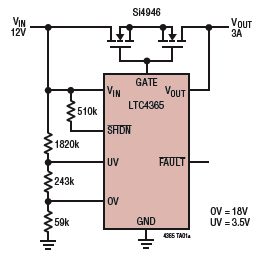
\includegraphics[width=0.5\textwidth]{images/ltc4365.png}
		\caption{LTC4365 application notes.}
	\end{centering}
\end{figure}
In this application the shut-down pin is always high, which makes the device open the MOSFETS if Vin is between the under voltage and over voltage threshold voltage.

Is necessary to define the over and under voltage threshold, this is found in the common requirements.\\
\\
Common requirements:\\\\
$V_{in} = 30V$ \\
$Offset = \pm 10\% $\\
\\
From the datasheet:\\\\
$ I_{UV} = 10nA $ \\
$ V_{OS} = 3mV $\\
\\
$V_{OSUV}$:maximum tolerable offset (error)\\
$I_{UV}$:worst case scenario current leakage.\\
\\
Under voltage requirement:\\\\
$ U_V=30V-(30*10\%)=27V $\\
\\
Over voltage requirement:\\\\
$ O_V=30V+(30*10\%)=33V $\\
\\
For working conditions of the device the bellow equation have to be true:\\\\
$ R_3+R_4=\frac{V_{OSUV}}{I_{UV}} $\\
\\
Using the formulas given in the datasheet to calculate the value of the 2 resistive dividers:\\\\
$ R_2 = 2*\frac{3mV}{10nA}*(27V-0.5V) = 15.9M\Omega $ Approximate 16M $\Omega $\\ 
\\
$ R_4 = \frac{\frac{V_{OSIU}}{I{UV}}+R_3}{2*O_V} = 246.97k\Omega $ Approximate 250k $\Omega $\\ 
\\
$ R_3 = \frac{V_{OSUV}}{I_{UV}}-R_1 = 50k\Omega $\\
\\
%
\lineparagraph{Simulations}
Linear Technologies have a simulator for their devices, the LTSpiceIV, is free software that can be downloaded from the web site.
Using LTSpice to simulate the behaviour of the LTC4365 with the required values for the power switch system.
%
\begin{figure}[H]
	\begin{centering}
		%\missingfigure{Updated timebox figure}
		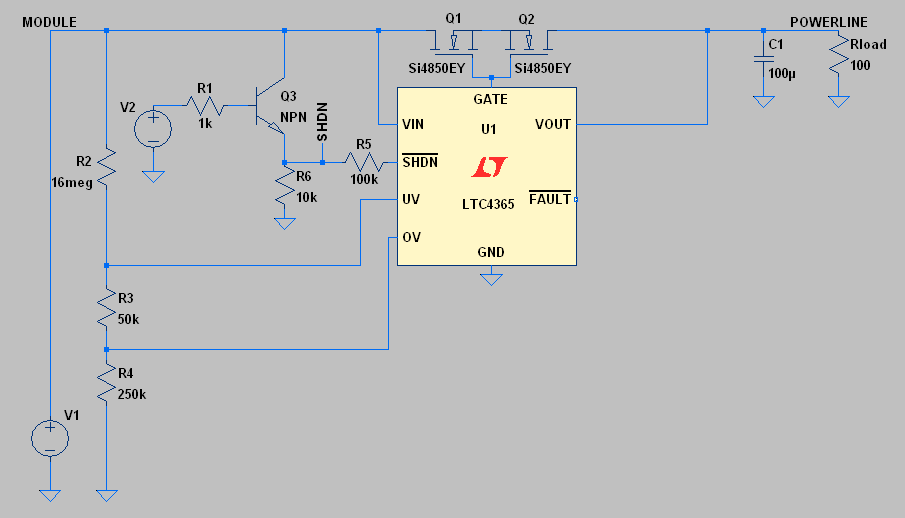
\includegraphics[width=1\textwidth]{images/tb5_LTC_simu1.png}
		\caption{Schematics for the device LTC4365}
	\end{centering}
\end{figure}
%
In the schematics a basic circuit is draw taken from the datasheet of the device, with a NPN transistor to drive the shut-down pin high and low. Two N-channel MOSFETs are connected back to back to  stop the voltage from passing to the load when the device is shut down. The system will work as power switching and ideal diode.
%
\lineparagraph{Case Scenario 1 ( Producer device connected to the MODULE side )}
\begin{figure}[H]
	\begin{centering}
		%\missingfigure{Updated timebox figure}
		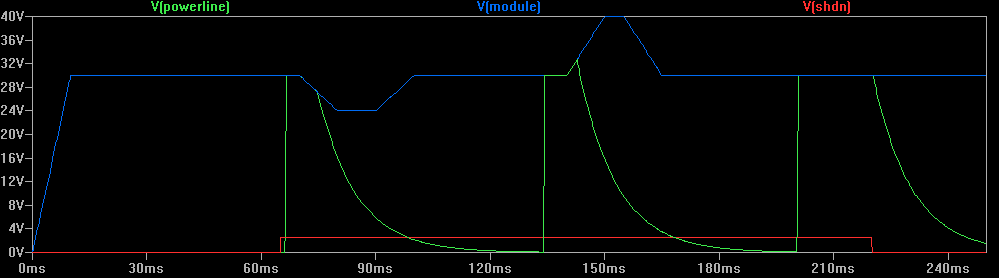
\includegraphics[width=1\textwidth]{images/tb5_LTC_case1.png}
		\caption{Simulation case scenario 1}
	\end{centering}
\end{figure}
In this case scenario the under voltage and over voltage can be tested along with the shut down pin. The simulation has a total time of 250ms, the system takes 10ms to stabilized at 30V which will stabilize the device at that voltage. At 65ms the NPN transistor is high, driven the input voltage to the shut down pin, with the shut down pin high the device will drive the gates for the two MOSFETs high and the current will flow through the MOSFETs from MODULE to POWERLINE as expected. 
The voltage at the module at 80ms is changed to 24V, this will test the under voltage threshold value. From the calculations made in the analysis section, the device should sink the gates to ground when the voltage is under 27V, this happens with success at 75ms as it can be seen in the simulation above.
To simulate over voltage protection, the MODULE (source) is set to 30V so the device can stabilize again. At 140ms the voltage is pull up to 40V, which the device should sink the gates of the MOSFETs when the voltage is 33V, this happens with success at 142ms.
To test the control of the shut down pin, the voltage on the source side is set to 30V, getting the device to stabilize again. With the device in working conditions the NPN transistor is turned off at 220ms, the shut down pin is then pull down by a 10k$ \Omega $ resistor.\\
%
\lineparagraph{Case Scenario 2 ( Device off, no energy flow from MODULE to POWELINE and the other way around )}
In the case scenario 1, there is no energy flowing when the device is off, is necessary now to simulate if the device is working as a diode, if no energy flows in the opposite direction. In this simulation the source and load positions are changed.
\begin{figure}[H]
	\begin{centering}
		%\missingfigure{Case 2 Schematics changed}
		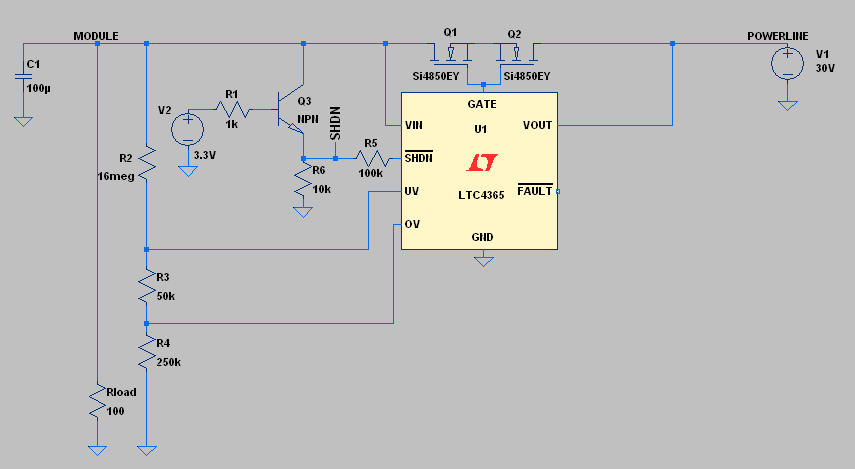
\includegraphics[width=1\textwidth]{images/tb5_LTC_simu2sc.png}
		\caption{Schematics for the device LTC4365 with Case scenario 2 specifications}
	\end{centering}
\end{figure}
%
Being now the POWERLINE the source and the MODULE the load, this situation can occurs when a battery is fully charged and there is a different potential higher on the POWERLINE side. The device is going to insure that no energy flows in the opposite direction. This is successfully shown in the simulation bellow.
%
\begin{figure}[H]
	\begin{centering}
		%\missingfigure{Case 2 Simulation}
		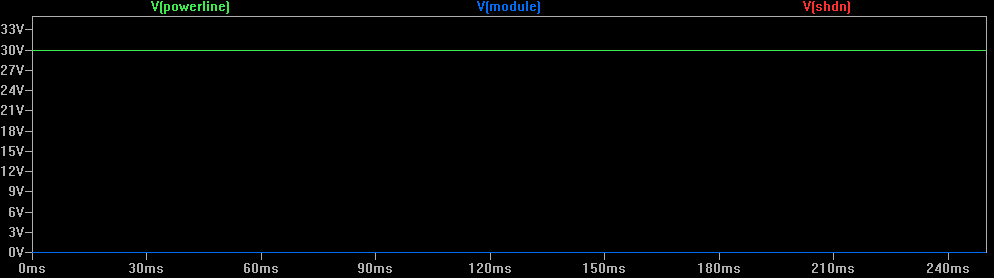
\includegraphics[width=1\textwidth]{images/tb5_LTC_simu2.png}
		\caption{Simulation for case scenario 2}
	\end{centering}
\end{figure}
%
The voltage at the source (POWERLINE) is kept at 30V, and at the load (MODULE) the voltage is around 0V (1mV), in this configuration the circuit is behaving as expected. When the device is off, and the energy flow in the opposite direction the system behave as a diode.
%
\lineparagraph{Current Sensors}	
%
Being part of a green energy system, a current sensor is implemented in this power switch system. The measurement of current allows the system to calculate the efficiency of each module connected to the switch port. The current measurements are shown to the user on the web interface.
%
The sensor used is a hall effect linear current sensor from Allegro, the ACS756SCA-050B, a bidirectional hall effect sensor with range from -50A to +50A.
%
\begin{figure}[H]
	\begin{centering}
		%\missingfigure{Updated timebox figure}
		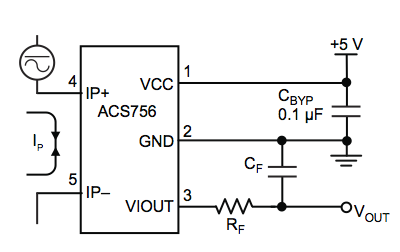
\includegraphics[width=0.5\textwidth]{images/current_sensor.png}
		\caption{ACS756SCA Typical application}
	\end{centering}
\end{figure}
%
A test for this device is set on a bread board, the measurements are made using a voltmeter on the output pin. At a temperature of $ 24^\circ C $ the output increments approximated 40mV for each ampere this can be matched with the datasheet. Since we can have a meaningful measure with the factory ranges, theres is no need to amplify the signal.
%
\begin{figure}[H]
	\begin{centering}
		%\missingfigure{Current sensor set up.}
		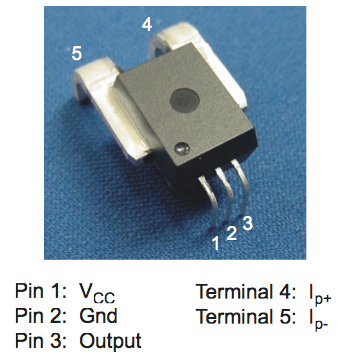
\includegraphics[width=0.40\textwidth]{images/tb5_CS_photo.png}
		\caption{ACS756SCA-050 pins.}
	\end{centering}
\end{figure}
%
\subsubsection{Design}
%
%	Design
%
%                UML/SysML deployment view(s)
%                Mechanical specifications and dimensioning
%                HW module specification per block
%                UML SW deployment view
%                Class specification
%                Refactored class diagram
%                Use case scenarios specifications
%                Sequence diagrams
%
The redesign of the power switch system required some more analysis since this is the main functionality of the energy hub. 
\lineparagraph{Power Switch Overview}
An overview of the system to be can be seen bellow.
%
\begin{figure}[H]
	\begin{centering}
		%\missingfigure{System Block Diagram}
		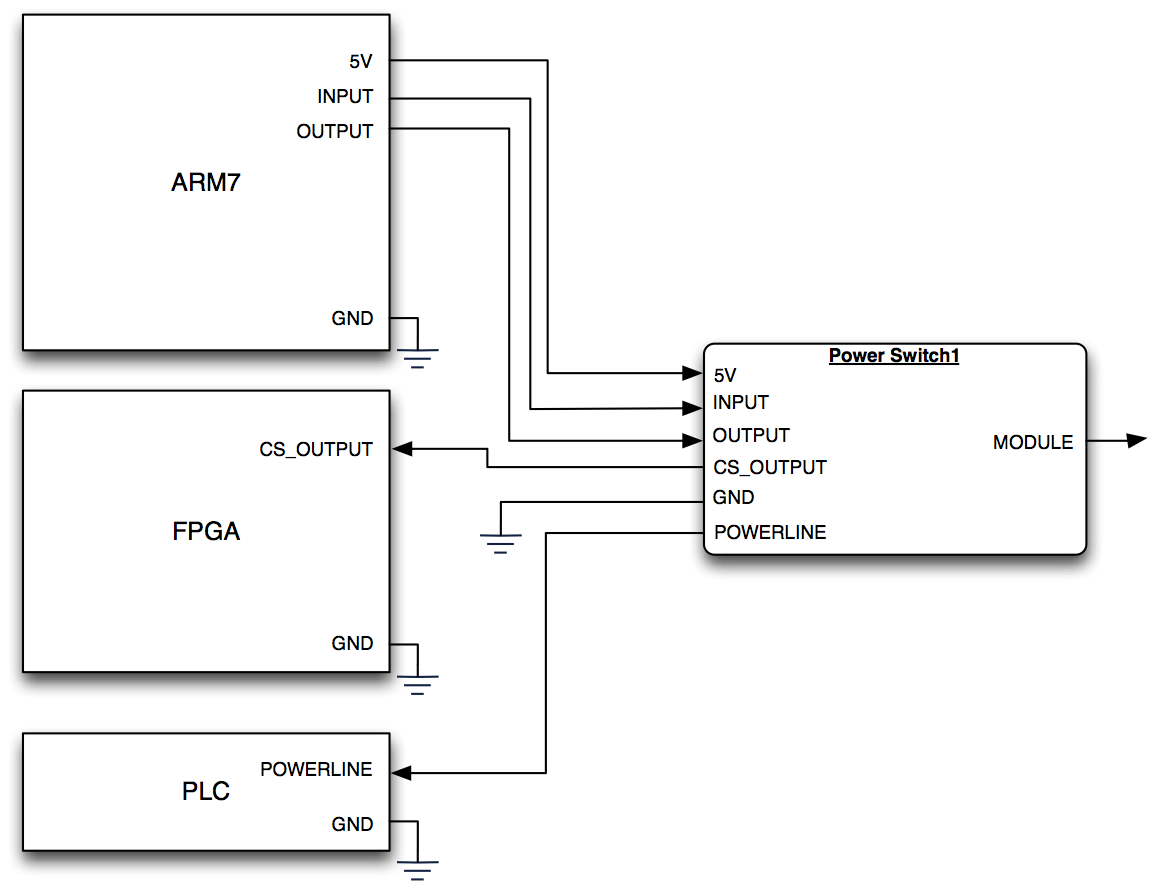
\includegraphics[width=0.90\textwidth]{images/PS_BlockDiagram.png}
		\caption{ACS756SCA-050 pins.}
	\end{centering}
\end{figure}
%
In this block diagram the connection between the different modules can be seen. The ARM7 controls the input and output pins of the power switch system, a device driver will be implemented for this functionality later on this project. 
The CS\_OUTPUT corresponds to the current sensor voltage output that goes from 0V(-50A) to 5V(50A), this is connected to one of the 8 ADCs implemented on the FPGA and retrieved to the core system (ARM7) through the EMC (External Memory Control) implementation.
POWERLINE pin form all power switch systems are connected to the same track into the PLC module. This will work as a sniffer fro new communication arriving and to send communication to the modules connected to the energy hub.
The module pin will is a connector for each module, in this prototype 4 ports are built, since there's no more than 4 modules in development.
%
\lineparagraph{Schematics}
Schematics of the power switch system bellow.
\begin{figure}[H]
	\begin{centering}
		%\missingfigure{Current sensor set up.}
		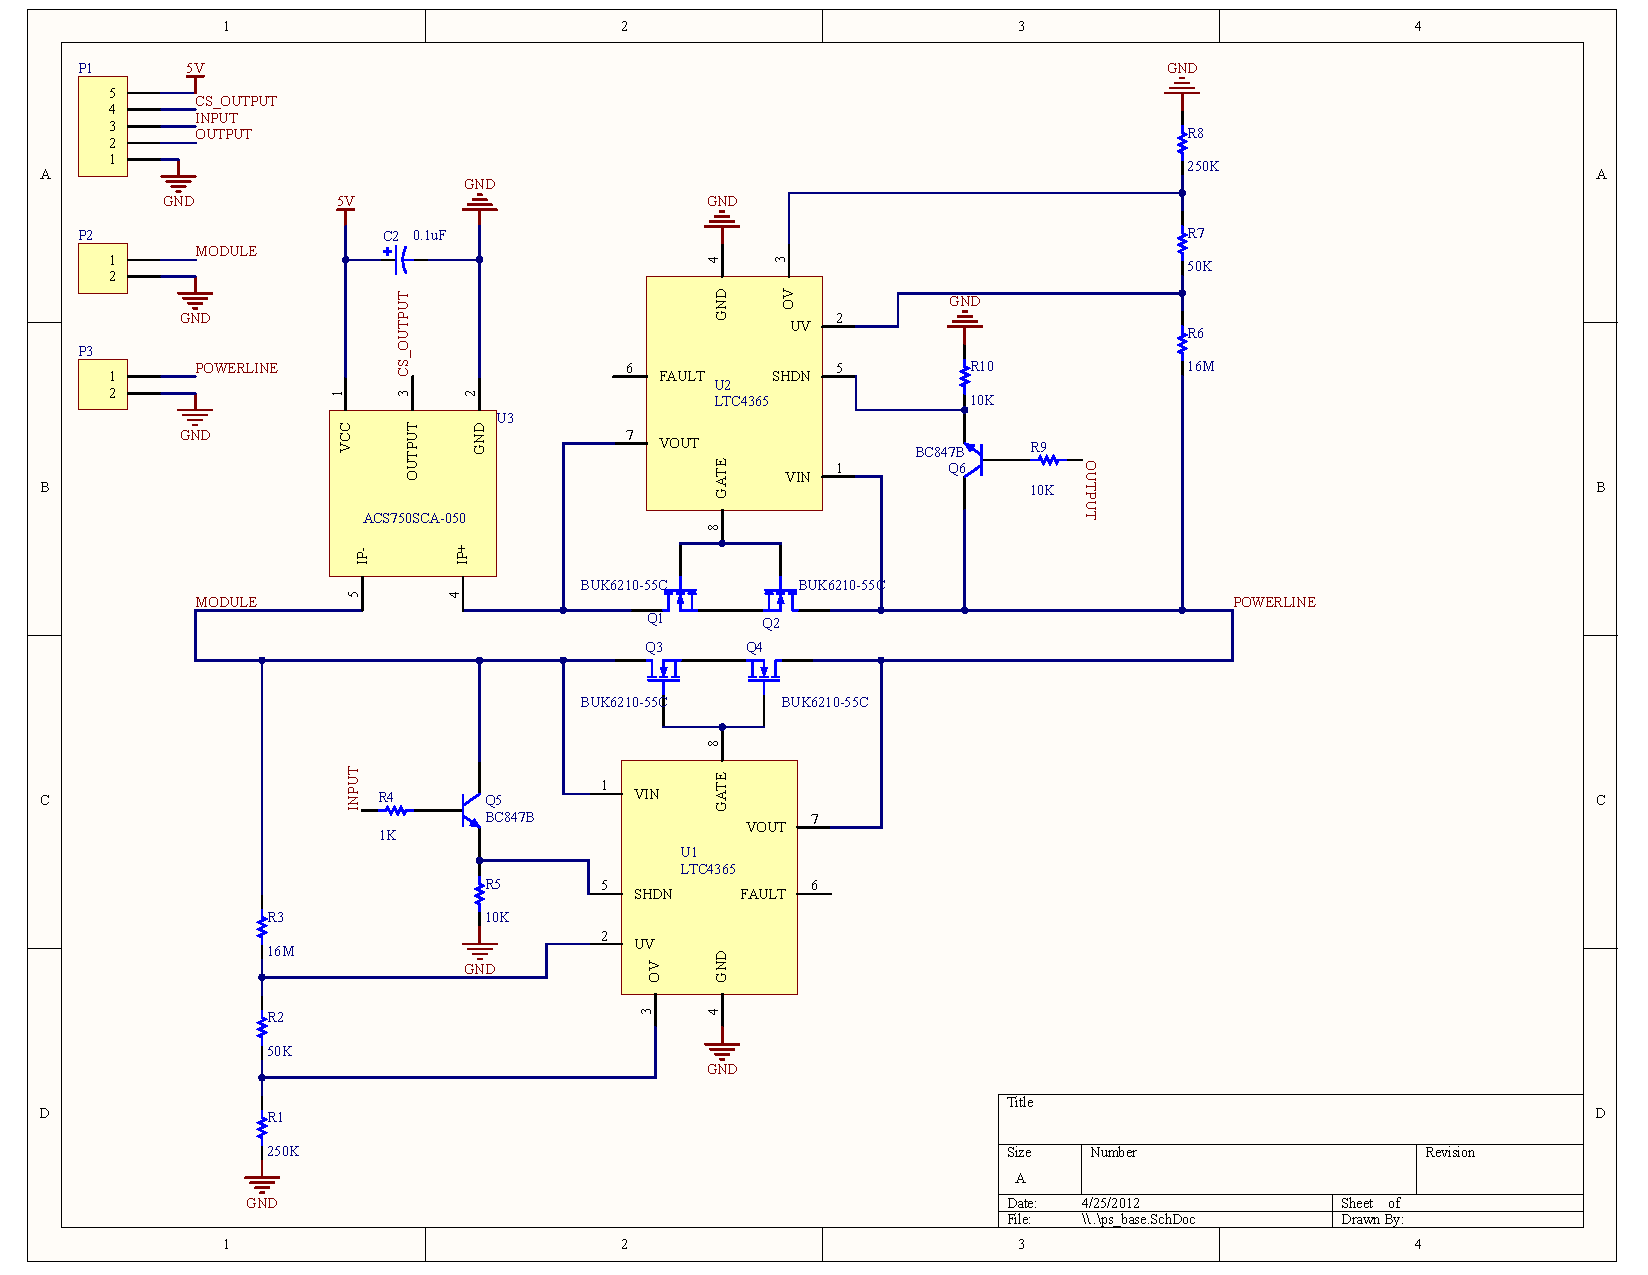
\includegraphics[width=1.0\textwidth]{images/PS_PCB.pdf}
		\caption{Power switch system schematics.}
	\end{centering}
\end{figure}
In this schematics the current sensor is add to the system a long with the new LTC4365 devices to control the two back to back N-channel MOSFETs. A NPN transistor is added between the $ V_{in} $ and the shut down pin, this will drive the pin to the input voltage or connect to ground, in case off power failure the power switch systems are disconnected since the shut down pin is pull down to ground through a 10K$ \Omega $ resistor.
\lineparagraph{PCB layout}
A layout is made using Altium Designer software version 10. This layout is a prototype so the components have more space between them for easier debugging and changes if necessary.
\begin{figure}[H]
	\begin{centering}
		%\missingfigure{PS layout image.}
		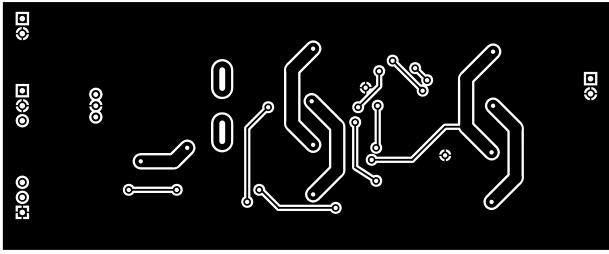
\includegraphics[width=1.0\textwidth]{images/tb5_layout_bottom.png}
		\caption{Power switch layout bottom layer.}
	\end{centering}
\end{figure}
\begin{figure}[H]
	\begin{centering}
		%\missingfigure{PS layout image.}
		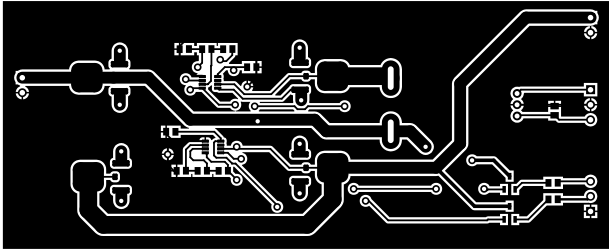
\includegraphics[width=1.0\textwidth]{images/tb5_layout_top.png}
		\caption{Power switch layout top layer.}
	\end{centering}
\end{figure}

The board is going to be assembled and tested in time box 6.

\subsubsection{Verification}
All the verifications for this board are changed to time box 6 since the PCB will not be ready at this moment:
\begin{table}[H]
\centering
	\begin{tabular}{| c | l | c |}
		\hline
		Verification & Description & Acceptance \\\hline
		1 & Switch the voltage as input or output & TimeBox6 \\\hline
		2 & Over voltage and under voltage are kept 30V $ \pm10\% $ & TimeBox6 \\\hline
		3 & Current between maximum 30A & TimeBox6 \\\hline
		4 & Power Line Communication through the switching system & TimeBox6 \\\hline
		5 & 4 PCB switching system & TimeBox6 \\\hline
	\end{tabular}
\end{table}
%
%	Verification
%
%                Module tests
%                Integration tests
%                Acceptance test
%%%%%%%%%%%%%%%%% Dennis Begin%%%%%%%%%%%%%%%%%%%%%%%%%%%%%%%%%%%
\subsection{Platform setup - Dennis} 
A virtual CentOS machine running on a machine at school has been assigned to each team in order to have a host machine where the boot loader (u-boot) can be compiled and modifications to the uClinux kernel can be made. Unfortunately the kernel compiled started to kernel panic. After undoing the different things done (removing files from the rc file and removing different kernel modules) the kernel kept panicking. Instead of using any more time on the machine, another similar virtual machine has been created on a local machine. The virtual machine is running CentOS 5.8 (like the one assigned), fortunately no kernel panic have been detected after compiling the kernel on the "new" local machine. Another benefit by having a local machine up and running is the flexibility as the Embedded Artist board should be connected to the schools network in order to access the tftp server where the board loads the kernel from throughout the development period. Now a tftp server has been set up on the local machine where to the development board can be directly connected though an ethernet cable.
\subsubsection{Network File system}
In order to speed up the development process of user space applications and device drivers to the board, a NFS server has been setup on the local host machine using the machintosh application \textit{NFS Manager}. The NFS disk is then mounted on the board by issuing the command: \\\textit{\#mount -o nolock,rsize=4096,wsize=4096 -t nfs 192.168.1.1:/Users/Shared/nfs\_mount /mnt/nfs}, 
\\which mounts the disk in \textit{/mnt/nfs}. When having the NFS server setup, there is no need to recompile the whole kernel when changes have been done to a kernel module or a user space application before it can be tested on the target. 

\subsection{UART Device driver - Dennis} 
As specified in the Technical platform section, the board used is LPC2478-32 from Embedded Artists. The on-board ARM processor is running uClinux, which is a Linux kernel for micro controllers without a memory management unit. In order to communicate with the UART hardware on the board a device driver has to be written, which is a piece of software that allows user-space applications in the kernel to interface with a hardware device (in this case the UART). The reason why implementing a UART driver, is to be able to communicate with the Power Line module which uses UART interface. 
\begin{table}[H]
\centering
	\begin{tabular}{|p{1.2cm}|p{2.3cm}|p{6cm}|p{6cm}|}
	\hline
	ID		& Requirement		& Description												& Comments\\\hline
	F-1.2		& Communication - System & The hub shall be able to communicate with a connected module through power line communication. & The interface to the power line module is UART.\\\hline
	\end{tabular}
\end{table}
%			Intro
%					verification specification
%					deployment specification
\subsubsection{Analysis}
The UART used for communication to the Power line module is UART2, however instead of making a device driver especially for UART2, a more generic driver is build instead so other UART can be used in the future if there is a need for it. 
\p On the 32 bit LPC2478 processor the UART1 is not supported and UART0 is used as console, so during initialization it is very important not to change in any registers concerning these, to avoid kernel panic or loose communication with the console.
\p The initial framework for the driver was made in the last time box, which will be used as the skeleton together with the bare metal UART driver also made in the last time box. 

%			Analysis
%
%                Refactored block diagram
%                Refactored class diagram
%                Detailed use cases
%                User interface specification
%                System interface specification
%                Dimensioning specification 
\subsubsection{Design}
Before implementing the kernel module, it has to be thought through how to operate with the module from the user side of it. A small test program has been created in order to have some implementation guide lines, but also to have a verification script to all the time test against, to check if the module fulfills all the tests. 
\p The script either opens the /dev/uart2 file and reads it, or opens it and writes the different commands available. After writing the file with one command, the content of the file is deleted (flushed) to prepare for a new operation. 
\begin{lstlisting}[language=c]
#define UART "/dev/uart2"

int main(int argc, char *argv[]) {
        FILE *fp;
	//Write commands
	char buffer1[] = {"INIT:8N1"};
	char buffer2[] = {"BAUD:9600"};
	char buffer3[] = {"WR:55"};
	char buffer4[] = {"WR:0x55"};
	char buffer5[] = {"help"};
	//read buffer
	char read[10];
	//If read is not specified in the arguments do a write
	if(strncmp("read", argv[1], 4) != 0){	//Open the file
		if ((fp = fopen(UART,"wb"))==NULL){
                	printf("Cannot open file.\n");
               	 	exit(0);
        	}
		//Initialize UART2 with 8N1 setup
		fwrite(buffer1, 1, sizeof(buffer1), fp);
		fflush(fp); //Empty the file
		//Define baudrate of devie
		fwrite(buffer2, 1, sizeof(buffer2), fp);
		fflush(fp);
		//Write a value decimal
 		fwrite(buffer3, 1, sizeof(buffer3), fp);
		fflush(fp);
		//Write a value hexadecimal
 		fwrite(buffer4, 1, sizeof(buffer4), fp);
		fflush(fp);
		//Write out different file options
 		fwrite(buffer5, 1, sizeof(buffer5), fp);
        	fclose(fp);
	}
	//Read the file
	else{
		if ((fp = fopen(UART,"rb"))==NULL){
                	printf("Cannot open file.\n");
               	 	exit(0);
        	}
		//Read the file and print it if something available
		if(fread(read,1,10,fp) > 0) printf("\nVAL: %s\n",read);
		else printf("\nFail or nothing to read\n");

		fclose(fp);
	}
        return 0;
}
\end{lstlisting}
As it can be seen in the code, the user has the ability to:
\begin{itemize}
	\item help - get a list of commands available in the kernel module.
	\item WR: - Write a character, which is transmitted on the UART module chosen. The value can be either hex or decimal.
	\item BAUD: - Change the baud rate of a UART to for instance 9600, 115200 or others.
	\item INIT: - Initialize the module with \textit{Word length}, 5,6,7 or 8 bits, \textit{stop bits}, 1 or 2 and \textit{parity bit} on or off. 
\end{itemize}
Note that the first time a device is opened after reset the INIT and BAUD shall be written to it in order to work as wanted. 
%        Design
%
%                UML/SysML deployment view(s)
%                Mechanical specifications and dimensioning
%                HW module specification per block
%                UML SW deployment view
%                Class specification
%                Refactored class diagram
%                Use case scenarios specifications
%                Sequence diagrams
\subsubsection{Implementation}
%%%%%%%%%File Descriptor%%%%%%%%%%%%%%%
As the device has to be able to both read and write, the file descriptor shall at minimum look like below with a open, close, read and write function. Further implementations is discussed in the conclusion section.
\begin{lstlisting}[language=c]
static struct file_operations uart_fops = {
	.owner   = THIS_MODULE,
	.read	 = uart_read,
	.write   = uart_write,
	.open    = uart_open,
	.release = uart_close,
};
module_init(uart_mod_init);
module_exit(uart_mod_exit);
\end{lstlisting}

%%%%%%%%%INIT/EXIT%%%%%%%%%%%%%%%
The init and exit functions are similar to the one used in the ADC, except that the UART2 and UART3 power pins are disable by default. If these pins are set and reset then the UART devices erases its settings. Therefore the power pins for UART2 and UART3 are set when inserting the module (UART0 and UART1 are enabled at reset).
\begin{lstlisting}[language=c]
m_reg_bfs(PCONP, 0x03000000);
\end{lstlisting}

%%%%%%%%%OPEN/CLOSE%%%%%%%%%%%%%%%
The open and close functions are almost similar to the skeleton made, except that the pins for a module is set the first time a file is opened. When the file closes the pins are not reset to GPIO's as it should still be able to receive data and put it into its buffer. 
\begin{lstlisting}[language=c]
static int uart_open(struct inode* inode, struct file* file){
	---
	if(chRefCnt[num] == 0){
		file->private_data = (void *) num;
		if(num == 0 || num == 2 || num == 3){
			m_reg_bfs(PINSEL0, enable_pinsel[num]);
		}
		else if(num == 1){
			m_reg_bfs(PINSEL7, enable_pinsel[num]);
		}
	}
	chRefCnt[num]++;
}
\end{lstlisting}

%%%%%%%%%%%READ%%%%%%%%%%%%%%%%%
As for now the read function is implemented as a dummy function which only returns a value when it is called. This implementation is similar to the one implemented in the bare-metal driver. This way of implementing a read call is very simple but also very inefficient. Further improvements of this is discussed in the conclusion section. 
\begin{lstlisting}[language=c]
static ssize_t uart_read(struct file *p_file, char *p_buf, size_t count, loff_t *p_pos){
	---
	if(endRead[num]){
		endRead[num] = 0;
		return 0;
	}

	if(!(m_reg_read(ulsr[num]) & 0x01)){
		return 0;
	}
	val = m_reg_read(urbr[num]);
	len = intToStr(val, p_buf+*p_pos, count, 10);
	if(len < count){
		p_buf[len++] = '\n';
	}
	endRead[num] = 1;

	return len;
}
\end{lstlisting}

%%%%%%%%%%%GET CMD%%%%%%%%%%%%%%%%
When writing to the file, four different valid commands can be given. The \textit{getCommand} function reads the string send and by comparing the string to a local array it returns a value to the write function, which handles the different commands given. 
\begin{lstlisting}[language=c]
static int getCommand(const char __user* buf, size_t count, char** ppArg){
	int i = 0;
	char* pEnd = NULL;

	if(strncmp("HELP", buf, 4) == 0 || strncmp("help", buf, 4) == 0){
		return HELP;
	}

	pEnd = strchr(buf, ':');
	if(pEnd == NULL)
		return INVALID;
	*ppArg = pEnd+1;

	for(i = 0; i < sizeof(commands)/sizeof(char*); i++){
		if(strnicmp(commands[i], buf, pEnd-buf) == 0){	
			return i;
		}
	}
	return INVALID;
}
\end{lstlisting}


%%%%%%%%%%%WRITE%%%%%%%%%%%%%%%%%
When the command has been read by the \textit{getCommand} function, the remaining length of the string is measured where after a function is called according to the return value of \textit{getCommand}. The help function writes out the different options of writing the file to the user. The write command first checks if the user has send a decimal or a hexadecimal value and then reads the value. Then the \textit{UART write busy flag} is checked to verify that the \textit{write register} is empty. If the register is not empty a value is counted up and returns a \textit{end of file} value (0) if the register is still not empty, otherwise it puts the value given into the \textit{write register}. The baud rate setup and init functions are explained below.
\begin{lstlisting}[language=c]
static ssize_t uart_write(struct file *filp, const char *bufp, size_t count, loff_t *p_pos){
	---
	cmd = getCommand(bufp, count, &arg);
	len = strlen(arg);
	
	switch(cmd){
	/********************************* HELP ********************************************/
	case HELP:
	    help();
	    break;
	/********************************* BAUD ********************************************/
	case BAUD:
	    baud = strToInt(arg, len, base);
	    set_baud(num,baud);
	    break;
	/********************************* INIT ********************************************/
	case INIT:
	    wl = strToInt(arg,1,1); arg++;
	    pb = strToInt(arg,1,1); arg++;
	    sb = strToInt(arg,1,1);
	    init_uart(num,wl,sb,pb);
	    break;
	/*********************************  WR  ********************************************/
	case WR:
	    if(strnicmp("0x", arg, 2) == 0){
	        arg += 2;
	        len -= 2;
	        base = 16;
	    }
	    val = strToInt(arg, len, base);
	    while(!(m_reg_read(ulsr[num]) & 0x20)){
	        ecnt++;
	        if(ecnt > 100)
	        return 0;
	    }
	    m_reg_write(uthr[num], val);
	    break;
	default:
	    printk("warning: invalid argument'\n");
 	}
  return count;
}
\end{lstlisting}

%%%%%%%%%%%INIT UART%%%%%%%%%%%%%%%%%
As written earlier, the init function has to be called the first time a file is opened after a reset (the same with the baud rate setup). The function enables the receive and transmit FIFO and sets up the: word length, amount of stop bits (1 or 2) and adds a parity bit if was requested. 
\begin{lstlisting}[language=c]
void init_uart(int dev, int wl, int sb, int pb){
	if(sb == 2) sb=1;
	else sb = 0;
	switch(dev){
	---
	/********** uart2 **********/
	case 2:
	    m_reg_write(U2LCR, 0x0);
	    m_reg_write(U2IER, 0x0);
	    m_reg_write(U2LCR, ( ((wl-5)<<0) |(sb<<2) | (pb<<3) ));
	    m_reg_write(U2FCR, 0x07);
	break;
	---
	}
}
\end{lstlisting}

%%%%%%%%%%%SET BAUD%%%%%%%%%%%%%%%%%
According to the lpc24xx data sheet\footnote{lpc24xx.user.manual.pdf, page 427} the UART clock must be 16 times the desired value of UART. From the drawing below it can be seen that the clock to the UART module is the same as the ARM7 clock (57.6MHz) as it is divided by one (these values are assigned to the PCLKSEL0 and PCLKSEL1 registers during low level initialization in u-boot). 
\begin{figure}[H]
	\begin{centering}
		%\missingfigure{Updated timebox figure}
		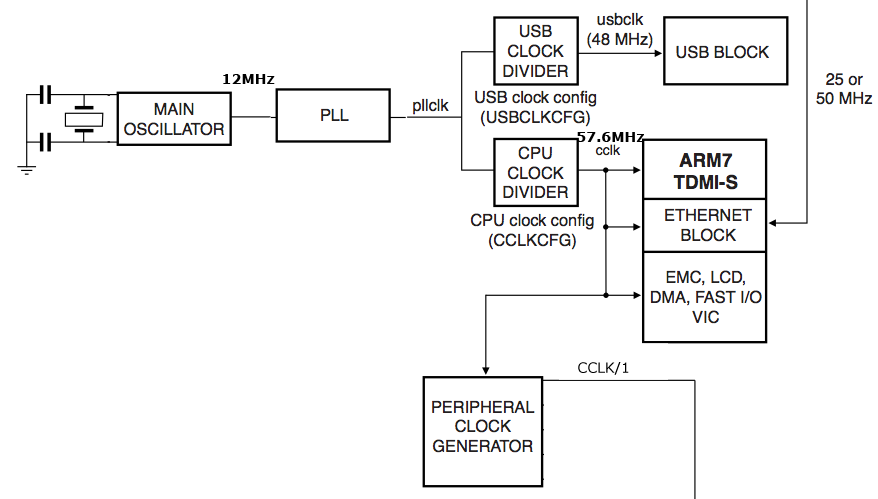
\includegraphics[width=0.7\textwidth]{images/peripheral_clock_gen.png}
		\caption{Peripheral clock to UART}
	\end{centering}
\end{figure}
In order to get the desired clock speed to the UART module, a scale value must be written to the \textit{Divisor Latch Register}.
\\If a baud rate of 9600 is wanted, the value written to the register must be: \\$57.600.000/(16*9600)=375$
\\As seen in the code below, the divisor register is split into two parts (a low and a high part).
\begin{lstlisting}[language=c]
void set_baud(int dev, unsigned int baud){
	switch(dev){
	---
	  case 2:
	    m_reg_write(U2DLL, (((LPC24xx_Fcclk/16)/baud) & 0xFF));
	    m_reg_write(U2DLM, (((LPC24xx_Fcclk/16)/baud) >> 8));
	  break;
	---
	}
}
\end{lstlisting}



The other functions used: \textit{intToStr}, \textit{strToInt}, \textit{chToUpper}, \textit{help} is code reuse from some of the other device drivers provided with the kernel: SFR, ADC and PWM.

%        Implementation
%
%                Mechanical drawings with details explained
%                Electronic diagrams with details explained
%                Source code with details explained
%                Description of integration 
\paragraph{Inserting the UART module in the kernel}
To automatically insert the module in the kernel during startup, a few files shall be made. The first thing to do is to create the different uart files in \/dev and specify that the module shall be inserted to the kernel after startup. The different files created is specified in the rc file. In the kernel folder structure the rc file used is placed in: \textit{/home/emb/uClinux-dist/vendors/EmbeddedArtists/LPC2478OEM\_Board}

\begin{lstlisting}[language=c]
---
/bin/mknod /dev/uart0 c 239 0 
/bin/mknod /dev/uart1 c 239 1
/bin/mknod /dev/uart2 c 239 2
/bin/mknod /dev/uart3 c 239 3
---
if [ -f /drivers/adc.ko ]; then
  insmod /drivers/adc.ko
fi
---
\end{lstlisting}
In the \textit{Makefile} in the same path a line shall be inserted to add the module to the \textit{romfs image} which is extracted during boot time. Also in the top, the value 5 shall be exchanged with 6, to indicate that there is an extra char device.
\begin{lstlisting}[language=c]
---
DEVICES = console,c,6,1
---
$(ROMFSINST) -S drivers/2.6.x/uart/uart.ko /drivers/uart.ko & \
---
\end{lstlisting}
The last thing to do is to add uart to the makefile in the drivers/2.6.x folder, to be sure that the kernel remakes the UART module when compiled if any changed were done. 
\paragraph{Adding the UART user space application}
When compiling a user space application through the kernel, there is no need to specify which gcc compiler to use or which flags to set in the different local Makefiles (this is all set in the big kernel Makefile). Therefore a makefile was found in the uClinux pdf book\footnote{Getting Started With uClinux Development A, page 72} in order to make small changes to the program, add it to the NFS folder and run it on the target, without the need for compiling the whole kernel and restarting the target each time. The makefile used:
\begin{lstlisting}[language=c]
CFLAGS= -Wall -W
LDFLAGS= -Wl,-elf2flt
CC= /usr/local/bin/arm-elf-gcc
RM=rm -f

PROG=uart
SRC= uart.c

OBJ=$(SRC:%.c=%.o)

$(PROG): $(OBJ)
	$(CC) $(CFLAGS) -o $(PROG) $(OBJ) $(LDFLAGS)

.PHONY: clean all dep

clean:
	$(RM) $(PROG) $(OBJ) *~ *.gdb .depend *.elf2flt *.elf
\end{lstlisting}
After finishing the application, it is added to the kernel by following the steps on Klaus wiki\footnote{\url{http://klaus.ede.hih.au.dk/index.php/How-to_add_a_user_space_application_to_uClinux}}.
\subsubsection{Verification}
The module is only verified with the UART2 hardware. The verification of the module is done by the UART user space application. At first the rx and tx pins where short-circuit, to make a loopback. After performing a write to the file by running the UART user space application, the file was read and the values compared to verify that the data was not corrupt. Afterward a test has been made similar to the one performed on the bare-metal driver, where the Embedded Artist board and an MBED communicates with each other through their own power line modules. 
%        Verification
%
%                Module tests
%                Integration tests
%                Acceptance test
\subsubsection{Conclusion}
The UART hardware can be accessed through the device driver, however, the efficiency of the module is not that good. Therefore the driver still need some improvements which shall be further added in order to get a better performance. 
\begin{itemize}
	\item Add interrupts to the receive part, to avoid reading the file once in a while to see if someone wrote anything.
	\item Add file write function, so a whole file can be compressed and sent to another module (wind turbine, photovoltaic, CAES or battery).
	\item Add more flexibility to initializing the module (break control, interrupt, ...) 
	\item Add more error handling and better feedback description if an invalid command is received.
\end{itemize}

%%%%%%%%%%%%%%%%% Dennis End%%%%%%%%%%%%%%%%%%%%%%%%%%%%%%%%%%%
\subsection{Interrupt register - Theis}
The interrupt register is made to tune performance by limiting the number of read statements the ARM7 is doing, in order to read from the Spartan 6. The interrupt register is not by itself fulfilling any requirements, but it is tuning the following: \textit{NF-1.5}\footnote{Requirement is found in table 3.2 in EPRO 3 project energy-hub} and \textit{B-3}\footnote{Requirement is found in table 3.4 in EPRO 3 project energy-hub}
\begin{table}[H]
\centering
	\begin{tabular}{|p{1.2cm}|p{2.3cm}|p{6cm}|p{6cm}|}
	\hline
	ID		& Requirement		& Description																& Comments\\\hline
	NF-1.5	& HW Interface		& 1 start button for the hub. 10 buttons to each start a module.			& It is only reading if the buttons state changes\\\hline
	B-3		& Errors			& Humidity and Temperature sensor will be placed inside the system housing	& The Spartan 6 interrupts if one of the following is happening\\\hline
	B-3.1	& Humidity			& If the humidity is above the maximum level 70\%, the system shuts down	& ARM7 only read on interrupt\\\hline
	B-3.2	& Temperature High	& If the temperature is higher than 55 degrees, the system shuts down		& ARM7 only read on interrupt\\\hline
	B-3.3	& Temperature Low	& If the temperature is below 0 degrees, the system shuts down				& ARM7 only read on interrupt\\\hline
	\end{tabular}
\end{table}
%			Intro
%					verification specification
%					deployment specification
\subsubsection{Analysis}
The purpose of the interrupt register is to limiting the number of readings the ARM7 is making from the Spartan 6. There is one interrupt pin routed from the AMR7 to the Spartan 6, but there is two blocks in the Spartan 6 that makes data for the ARM7. These blocks are the switch input block and the analog to digital converter\footnote{ADC} block. One way to use the interrupt is to allow the switch block to interrupt when a user interact with the system, and then read the ADC with a specific time interval. But to avoid to many unnecessary readings of the ADC, the interrupt register is the only block that is allow to interrupt the ARM7, the interrupt register gets interrupt signals from the ADC and the switch blocks, the register is arranging the interrupt, and when the ARM7 is interrupted, it reads data from the register to find out which block it should read.
\begin{figure}[H]
	\begin{centering}
		%\missingfigure{Updated timebox figure}
		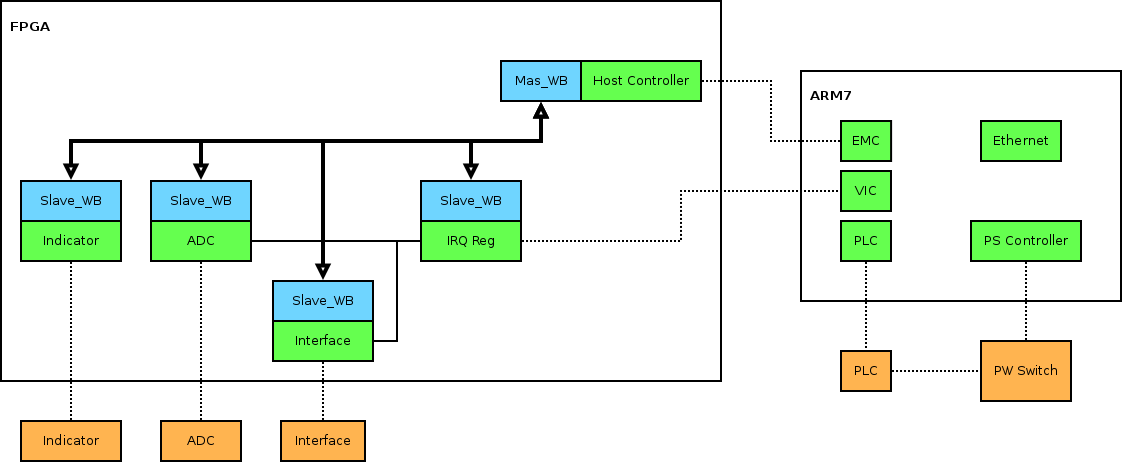
\includegraphics[width=1.0\textwidth]{images/tb5_modules_design.png}
		\caption{Module design with IRQ register}
	\end{centering}
\end{figure}
When a block sends an interrupt to the IRQ\footnote{Interrupt Request} register, it locates the interrupt and put the address to the block on to a FIFO\footnote{First In First Out}, and sends an interrupt to the ARM7, then the AMR7 read the FIFO to get the address on the interrupting block, in that way the ARM7 knows where to read next.
%			Analysis
%
%                Refactored block diagram
%                Refactored class diagram
%                Detailed use cases
%                User interface specification
%                System interface specification
%                Dimensioning specification 
%
\subsubsection{Design}
The purpose of the interrupt register is to make interrupt functionality on several block with only one interrupt pin to the ARM7. The interrupt register shall be optimized to wishbone use. The interrupt register without wishbone has to inputs, a vector of size N\footnote{N = number of blocks that is allow to interrupt} and an array that is N bit high and AddrRange\footnote{Wishbone address range} bit wide. The output is the IRQ pin to the ARM7 and a data vector equal to the wishbone data width. This is shown in the figure below.
\begin{figure}[H]
	\begin{centering}
		%\missingfigure{Updated timebox figure}
		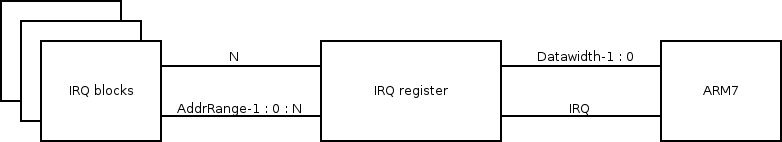
\includegraphics[width=1.0\textwidth]{images/tb5_irq_reg_nowb.png}
		\caption{IRQ register without wishbone}
	\end{centering}
\end{figure}
When a block needs to make an interrupt, it puts the wishbone address onto the input array to the IRQ register, and then sets the interrupt output high to tell the IRQ register that there is a valid address that needs to be read. The IRQ register save the address and interrupt the ARM7. When an interrupt occurs on the ARM7, it read the IRQ register to get the address that it shall read next, in this way it takes two wishbone read cycles for the ARM7 to get the right data, but the ARM7 is only reading if the Spartan 6 have valid data to read, instead of make reading with specific interval. The IRQ register save the interrupt in a FIFO in case interrupt is made faster than the ARM7 can read.\\
\paragraph{Interrupt output}
The interrupt output is set low as long a the FIFO is not empty, to tell the ARM7 to keep on reading till the FIFO is empty and sets the IRQ high again.
\paragraph{Data output}
The data output is equal to the wishbone data width, in this case it is 16 bit, and the address is 7 bit. The seven lowest data bits is used for the address to the block that sends the interrupt, the rest of the bits can be used for extra data from the IRQ register.
\begin{figure}[H]
	\begin{centering}
		%\missingfigure{Updated timebox figure}
		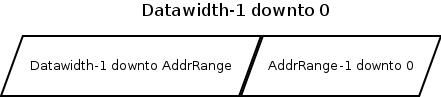
\includegraphics[width=0.55\textwidth]{images/tb5_irq_reg_data_o.png}
		\caption{IRQ register data output}
	\end{centering}
\end{figure}
%        Design
%
%                UML/SysML deployment view(s)
%                Mechanical specifications and dimensioning
%                HW module specification per block
%                UML SW deployment view
%                Class specification
%                Refactored class diagram½
%                Use case scenarios specifications
%                Sequence diagrams
%
\subsubsection{Implementation}
A block diagram for the interrupt register is shown below. It consist of three block for handling the interrupt, a input block which handled the input and write data to the FIFO. The FIFO act like memory for the interrupt data, and sends a interrupt to the ARM7. The output block takes input from the wishbone and handle the data to the wishbone, form the FIFO.
\begin{figure}[H]
	\begin{centering}
		%\missingfigure{Updated timebox figure}
		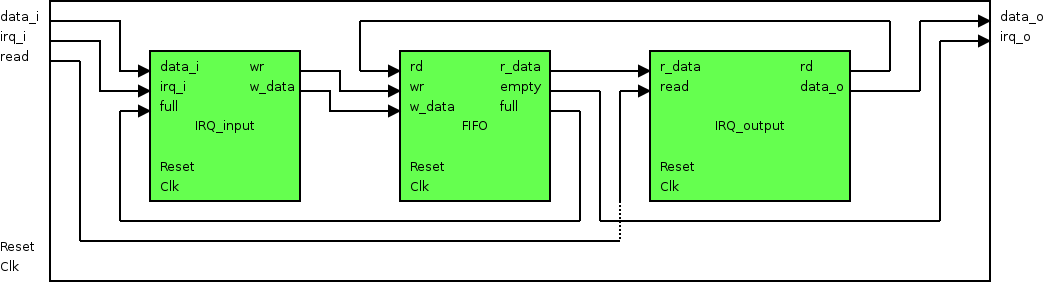
\includegraphics[width=1\textwidth]{images/irq_reg_block_dia.png}
		\caption{Block diagram for the IRQ register}
	\end{centering}
\end{figure}

\paragraph{FIFO - First In First Out}
The FIFO buffer is where the interrupt data is stored before they a read. The input block write data into it, and the output block read data out of it. The FIFO is necessary if the Spartan6 make interrupt faster than the ARM7 can read them. The figure below shows how the First In First Out principle is working.
\begin{figure}[H]
	\begin{centering}
		%\missingfigure{Updated timebox figure}
		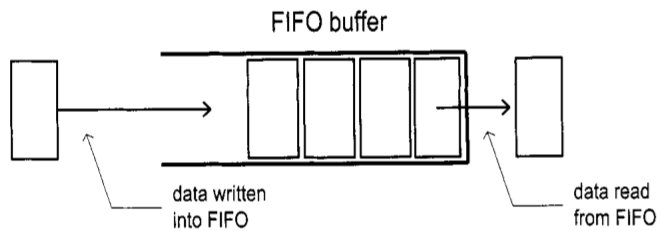
\includegraphics[width=0.6\textwidth]{images/tb5_fifo.png}
		\caption{Conceptual diagram of a FIFO buffer}
	\end{centering}
\end{figure}
The FIFO buffer code is from the book \textit{FPGA Prototyping by VHDL Examples - Listing 4.20}. It is a standard FIFO buffer, with a data vector input, an input for read and one for write, plus clock and reset. As output there is a data vector equal to the input vector, further more there is an empty and a full signal to indicate if the buffer is empty or full. A block diagram for the FIFO buffer is shown below.
\begin{figure}[H]
	\begin{centering}
		%\missingfigure{Updated timebox figure}
		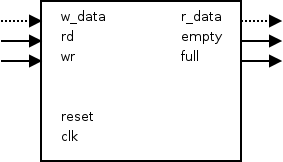
\includegraphics[width=0.45\textwidth]{images/tb5_fifo_block.png}
		\caption{State diagram for input}
	\end{centering}
\end{figure}
The FIFO buffer is used to hold the interrupt data from the other blocks in order to present it for the ARM7 in the right order.
\paragraph{IRQ input}
The input block gets data and interrupt input from every block with interrupt permissions in the system. The purpose of the block is to handle which block is interrupting and which data that have to be written to the FIFO in order to be handle by the ARM7 in the right way. Below the state diagram of the input block is shown. The purpose of a state digram is to make the coding easier.\\
When in IDLE the FIFO write is set low, the interrupt inputs is check, if non of them is high the interrupt counter is set low, to enable new interrupts. If a interrupt is high the state is change to IRQx, where the data output to the FIFO is set to the data from the interrupting source, after that is checks if it is the first time this data is written to the FIFO, if that is the case, the data is written to the FIFO and the returns to IDLE. 
\begin{figure}[H]
	\begin{centering}
		%\missingfigure{Updated timebox figure}
		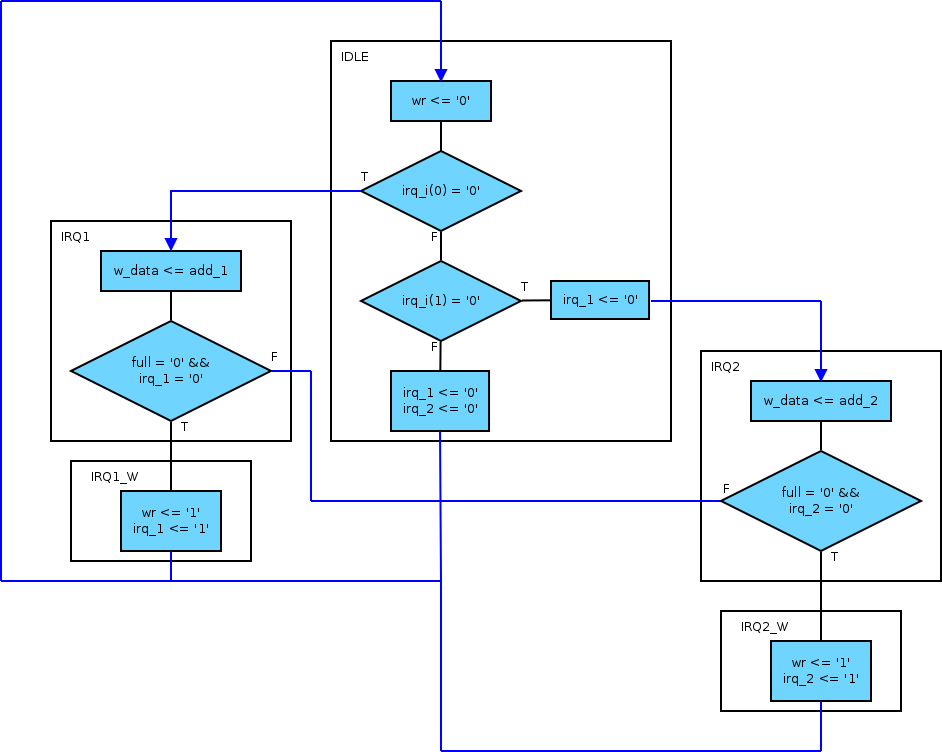
\includegraphics[width=0.9\textwidth]{images/tb5_irq_input_state.png}
		\caption{State diagram for input}
	\end{centering}
\end{figure}
In the code below the states are defined, this is easily done from the state diagram, the signals that can have the different states a value is also defined here.
\begin{lstlisting}[language=VHDL]
...
	--Types
	type state_type is	(
								IDLE,
								IRQ1,
								IRQ1_W,
								IRQ2,
								IRQ2_W
								);
	--Signals
	signal state_reg		: state_type;
	signal state_next		: state_type;
	signal irq_1				: std_logic		:=	'0';
	signal irq_2				: std_logic		:=	'0';
...
\end{lstlisting}
This code is where the states are set, if reset is active the state is set to IDLE else the state is set to state\_next.
\begin{lstlisting}[language=VHDL]
...
	-- state register
	process(Clk, Reset)
	begin
		if	(reset = '1') then
			state_reg		<= IDLE;
		elsif (Clk'event and Clk='1') then
			state_reg		<= state_next;
		end if;
	end process;
...
\end{lstlisting}
This is the part of the code where the state digram is implemented. A case statement is made with the state value as input. First the IDLE state is defined, here wr is set low, then it check if there is a interrupt, if that is the case then it sets the state to IRQx which sets the data and then check if it is first time the data is written else it just sets the state to IDLE, if it is first time the state is set to IRQx\_W where it write the data into the FIFO.
\begin{lstlisting}[language=VHDL]
...
	-- next state/output logic
	process(state_reg, irq_i, add_1, add_2, full, irq_1, irq_2)
	begin
		state_next		<= state_reg;
		--wr					<= '0';
		case state_reg is
		-- Idle state -------------------------------------------
			when IDLE =>
				wr		<= '0';
				if(irq_i(0) = '1') then
					state_next		<= IRQ1;
				elsif(irq_i(1) = '1') then
					irq_1					<= '0';
					state_next		<= IRQ2;
				else
					irq_1		<= '0';
					irq_2		<= '0';
				end if;
		-- IRQ1 state -------------------------------------------
			when IRQ1 =>
				w_data				<= add_1;
				state_next		<= IRQ1_W;

			when IRQ1_W =>

				state_next		<= IDLE;
				if((not full and not irq_1) = '1') then
					wr			<= '1';
					irq_1		<= '1';
				end if;
		-- IRQ2 state -------------------------------------------
			when IRQ2 =>
				w_data				<= add_2;
				state_next		<= IRQ2_W;

			when IRQ2_W =>

				state_next		<= IDLE;
				if((not full and not irq_2) = '1') then
					wr			<= '1';
					irq_2		<= '1';
				end if;
		end case;
	end process;
...
\end{lstlisting}

\paragraph{IRQ output}
The output block is reading the data out of the FIFO and present them for the wishbone. It gets a read input from the wishbone, when the ARM7 wants to read data from the register. The main purpose of the block is to make sure that the wishbone read the write data, and it is only reading once from the FIFO.\\
A state diagram for the output block is shown below. In the IDLE state rd is set low, then et check if the wishbone wants to read, else it reset the read counter, if the wishbone wants to read, the IDLE state checks if it is the first time by checking the read counter, if it is the first time the rd is set high to get the next data from the FIFO, and the read counter is set to one.
\begin{figure}[H]
	\begin{centering}
		%\missingfigure{Updated timebox figure}
		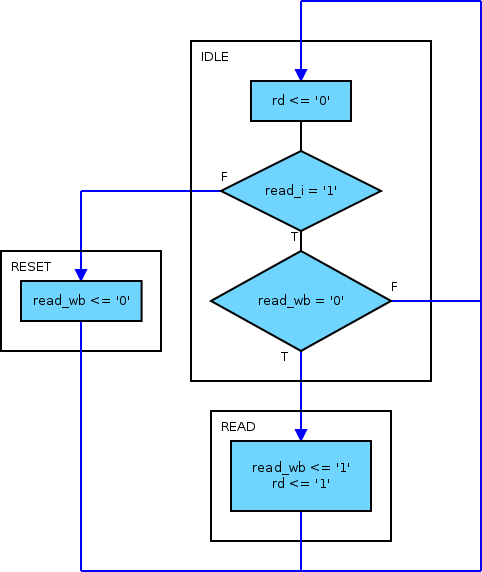
\includegraphics[width=0.55\textwidth]{images/tb5_irq_output_state.png}
		\caption{State diagram for output}
	\end{centering}
\end{figure}
Here the states is defined plus the read counter.
\begin{lstlisting}[language=VHDL]
...
	--Types
	type state_type is	(
											IDLE,
											READ_O,
											RSET
											);
	--Signals
	signal state_reg		: state_type;
	signal state_next		: state_type;
	signal read_wb			: std_logic;
...
\end{lstlisting}
The lower bits in the data\_o is set to the data from the FIFO, the other bits is set to zero. In the process the next state is loaded.
\begin{lstlisting}[language=VHDL]
...
	data_o(Datawidth-1 downto AddrRange)	<= (others => '0');
	data_o(AddrRange-1 downto 0)					<= r_data;

	-- state register
	process(Clk, Reset)
	begin
		if	(reset = '1') then
			state_reg		<= IDLE;
		elsif (Clk'event and Clk='1') then
			state_reg		<= state_next;
		end if;
	end process;
...
\end{lstlisting}
Below the state actions is defined following the state diagram. The rd is set low in IDLE and the wishbone read is checked. In READ the read counter is set to one and rd is set high to read data out of the FIFO.
\begin{lstlisting}[language=VHDL]
...
	-- next state/output logic
	process(state_reg, read_i, r_data, read_wb)
	begin
		state_next	<= state_reg;
		rd					<= '0';
		read_wb			<= read_wb;
		case state_reg is
		-- Idle state -----------------------------------------------------
			when IDLE =>
				rd		<= '0';
				if	(read_i = '1') then
					if	(read_wb = '0') then
						state_next		<= READ_O;
					else
						state_next		<= IDLE;
					end if;
				else
					state_next		<= RSET;
				end if;
		-- READ_O state ---------------------------------------------------
			when READ_O =>
				state_next		<= IDLE;
				read_wb				<= '1';
				rd						<= '1';
		-- RSET state -----------------------------------------------------
			when RSET =>
				state_next	<= IDLE;
				read_wb			<= '0';
		end case;
	end process;
...
\end{lstlisting}

\paragraph{Wishbone interface}
In order to use the interrupt register in the system, is shall be implemented as a wishbone slave, with a wishbone interface, this is done in the code below. The error and retry bit i set to zero, the acknowledge bit i set then the strobe input and the cycle input is high. In the process a synchronous reset is made. If the reset is inactive, it checks if the strobe and cycle input is high and the write enable is low, the meaning is to check if the wishbone wants to read or write. This module is a read only so it is not reacting on a write statement. If the wishbone wants to read, the data output is set and a read to the output block is set high, when the wishbone determinates the read cycle the data output is set to zero and the read statement for the output block is set low again.
\begin{lstlisting}[language=VHDL]
...
-- =================================================
-- WishBone logic
-- =================================================
	--  Concurrent assignments
	--	Wishbone cycle acknowledge
	err_o <= '0';	--error signal
	rty_o <= '0';	--retry signal
	ack_o <= stb_i and cyc_i;  --! asynchronous cycle termination is OK here.
	--Wishbone read
	data_output	:	process(clk_i)
	begin
		if(clk_i'event and clk_i = '1') then
			if(rst_i = '1') then
				dat_o <= (others => '0');
			else
				if((cyc_i and stb_i and not we_i) = '1') then
					case adr_i is
						when WBS_REG1 =>
							dat_o		<= data_o;
							read_i	<= '1';
						when others =>
					end case;
				else
				dat_o		<= (others => '0');
				read_i	<= '0';
				end if;
			end if;
		end if;			
	end process;
...
\end{lstlisting}
%        Implementation
%
%                Mechanical drawings with details explained
%                Electronic diagrams with details explained
%                Source code with details explained
%                Description of integration 
%
\subsubsection{Verification}
The verification of the IRQ register is made in a VHDL test bench, because there is currently no blocks with interrupt ability implemented. The verification test bench is shown below. The test is made by make four interrupts, this can be seen on the \textit{IRQ\_in} signal which has four pulses on the two signals. The address on \textit{add\_1} and \textit{add\_2} is written into the FIFO. The test bench also shows that the \textit{IRQ\_out} change after the first interrupt is assigned. After this four wishbone reads are made, by setting the cycle and the strobe input high, this give a acknowledge bit, and the \textit{Data\_out} is change to the first element in the FIFO, and the next read get the next data and further on. After the last wishbone read the FIFO is empty and the \textit{IRQ\_out} is set high again to indicate there is no interrupt.
\begin{figure}[H]
	\begin{centering}
		%\missingfigure{Updated timebox figure}
		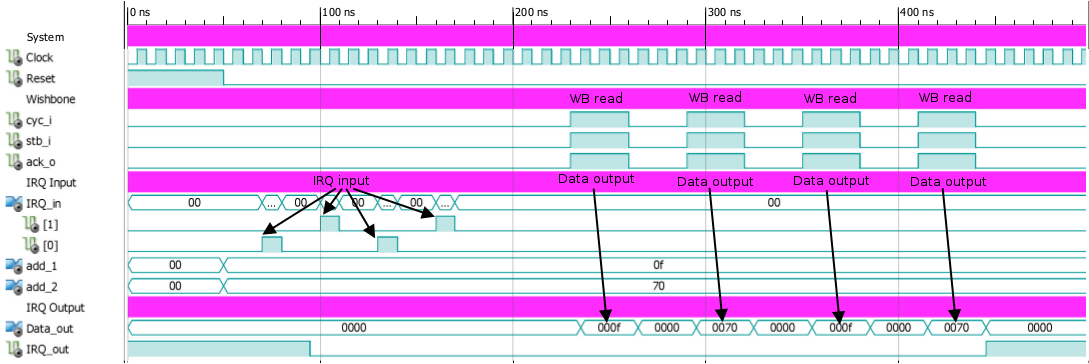
\includegraphics[width=1.0\textwidth]{images/tb5_irq_reg_testbench1.png}
		\caption{Test bench for the interrupt register}
	\end{centering}
\end{figure}
%        Verification
%
%                Module tests
%                Integration tests
%                Acceptance test
\subsubsection{Conclusion}
The test bench verify that the interrupt register is working with virtual signals in simulation. The switch block is to be change to have interrupt ability, and then it shall be implemented with the interrupt register and tested properly with communication and interrupt to the ARM7


\subsection{Deployment}
\paragraph{UART Device Driver}
The first version of the Device Driver is up and running (v0.1), which has implemented read and write functionality (non interruptible). Also different write calls have been implemented in order to initialize a channel.
\paragraph{Power Switch}
The power switch system is under development, 4 of this modules will be developed and a test bench build using fast prototyping tools. In time box 6 the complete development of this main system will be finish and a prototype will be present to the client.
	%which versions of the prototype the customer will get
	%with what functionality.
\paragraph{Interrupt register}
The interrupt register works in a test bench with wishbone interface. The implementation in the Spartan 6 is the next step and, interrupt ability is to be added to the switch block.
	%which versions of the prototype the customer will get
	%with what functionality.